
\begin{figure}[t]
\begin{center}
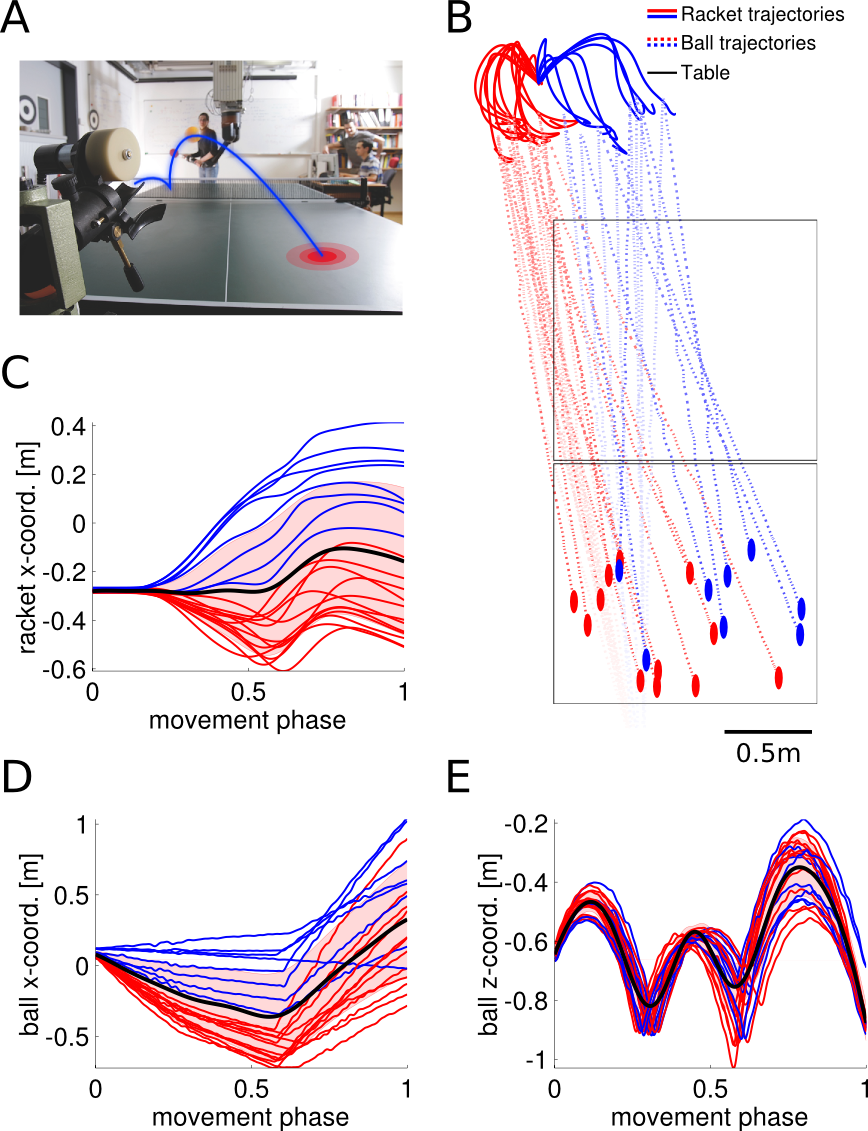
\includegraphics[width=0.8\columnwidth]{PingPong_Data.png}
\end{center}
\caption{(A-B) Trajectory prediction task in a table tennis setting using $20$ end-effector and ball trajectories. 
(C-E) Learned distributions over trajectories for three dimensions (out of six) using ProMPs. 
The colors (red and blue) are only used to visualize differences in the movement directions.
\label{fig:pingpong_data_promps}
}
\vspace{-0.5em}
\end{figure}


\begin{figure}[t]
\begin{center}
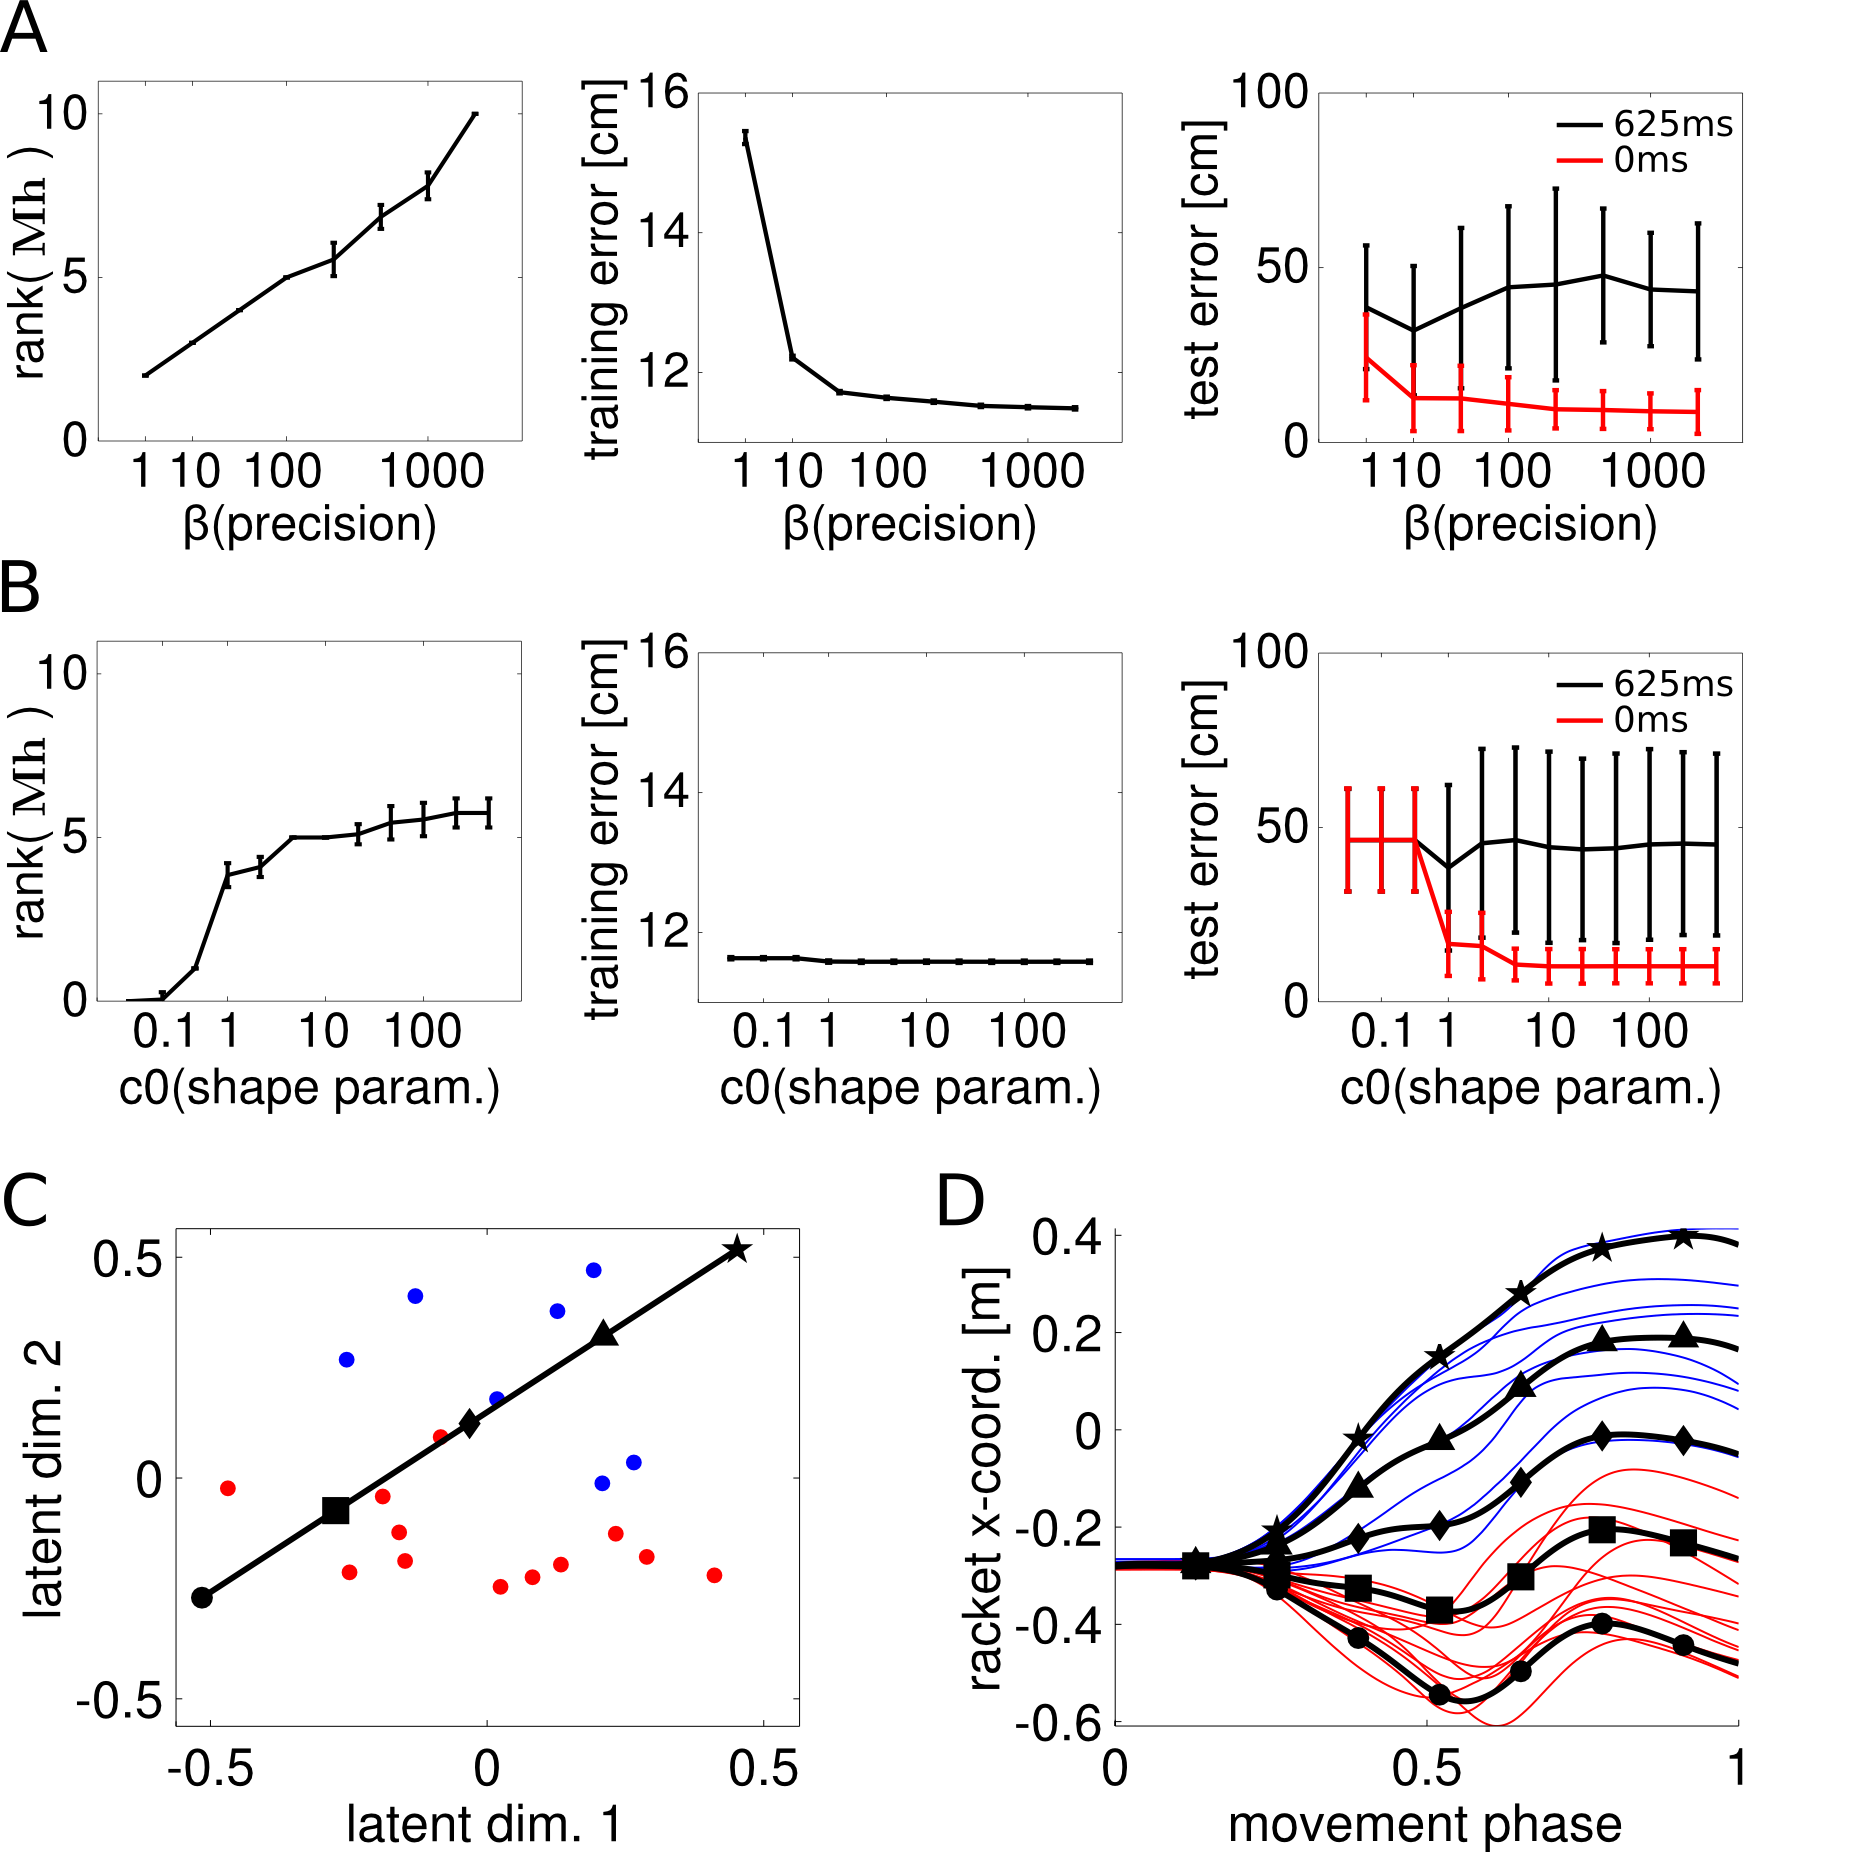
\includegraphics[width=\columnwidth]{PingPong_Robustness.png}
\end{center}
\caption{(A) The data precision parameter $\beta$ can be used to adapt the model complexity while avoiding overfitting (shown in the $2$nd and $3$rd panel for two planning horizons until the ball impact). 
(B) The gamma prior on the precision parameters $\lambda$ to increase the numerical stability has little effect on the prediction performance (for $c_0 \ge 1$). 
(C) Investigation of the effect of the latent variables, where the first dimension of $\textbf{h}$ describes the slope whereas the second dimension relates to the waviness (D).
\label{fig:pingpong_model}}
%\vspace{-0.5em}
\end{figure}

\section{Results}

We evaluate our method on two real robot tasks. In the first task the robot
played a table tennis game and we recorded the Cartesian coordinates of a
racket mounted at its end-effector and the Cartesian coordinates of the ball. 
A Barrett WAM anthropomorphic arm was used for this experiment~\cite{Muelling2011}. 
The robot provides regular updates about its
joint positions at a rate of 1KHz that are used by the forward kinematics to
compute the Cartesian position of the racket. The ball is tracked by a
high-speed, multi-camera vision system~\cite{Lampert2012} that provides updates
at a rate of 200Hz. The extracted dataset contains twenty ball and racket
trajectories. 

In the second task we placed an obstacle in front of a KUKA lightweight arm and 
demonstrated by kinesthetic teaching different ways to approach a desired
target point in Cartesian space. During the demonstrations we avoided hitting
the obstacle and we bypassed it either by moving to the left or to the right. The
demonstrations are depicted in Fig.~\ref{fig:bimodal_data_promps}. For this
experiment we recored the Cartesian position and orientation of the
end-effector. The state vector $\vec y_t$ for this experiment is seven
dimensional, three dimensions for the position and four for the quaternion based
orientation. 

%include time sync?

\begin{figure*}[!t]
\begin{center}
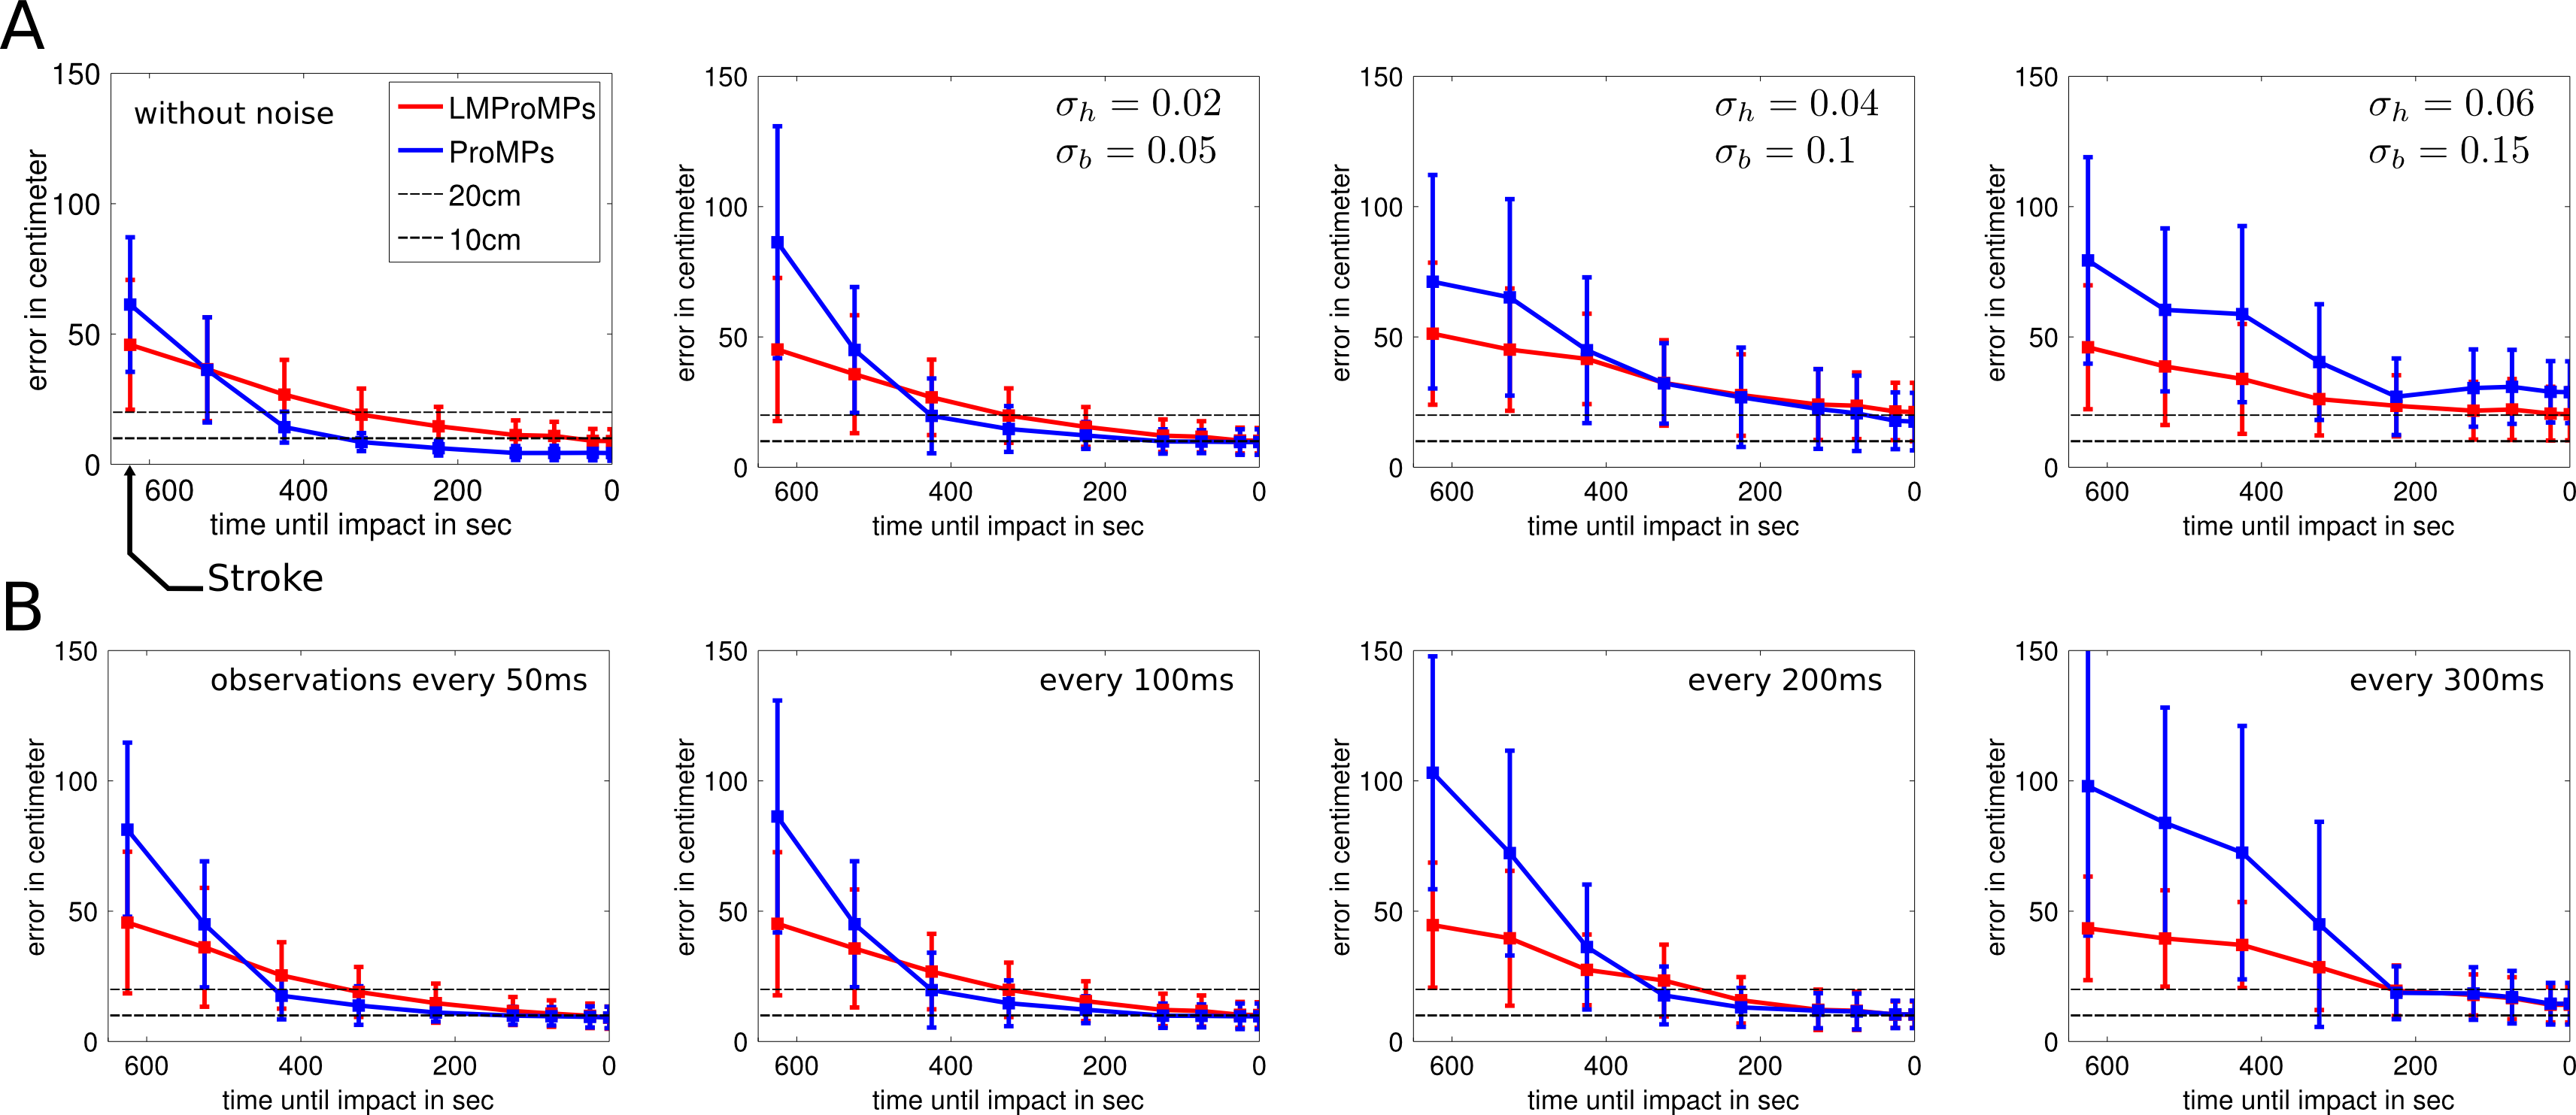
\includegraphics[width=0.8\textwidth]{PingPong_Overfitting.png}
\end{center}
\caption{The effect of noise (A) and missing data (B) on the prediction performance of ProMPs (blue lines) and LM-ProMPs (red lines).  
In (A), from left to right the amount of applied noise is increased. 
In (B) four different frame rates of observations ($\in \{50, 100, 200, $ and $ 300\}$ms) are investigated.
\label{fig:pingpong_overfitting}}
%\vspace{-0.5em}
\end{figure*}

\subsection{Summary of the investigated features}

We compare the proposed model, denoted as Latent Manifold ProMPs (LMProMPs) in the figures, 
to the standard ProMP approach in the two robotic setups. 

In the table tennis
scenario we investigate the effect of noise and missing data on predicting the
final ball impact location at the opponent's side of the table and we
demonstrate how the learned latent variables can be used to semantically analyze 
the data. 

Additionally, we demonstrate the beneficial properties of the mixture model
in representing the bi-modal distribution 
required to successfully execute the KUKA reaching task. We use the learned mixture model 
to generate trajectories to new target locations, not encountered during training, and execute
them on the real robot. We demonstrate that our proposed approach
successfully avoids the obstacle, while the standard ProMPs average over the two
modes and the generalization fails.


In both experiments we used linear regression to compute the feature weights
$\vec w$ and we subsequently applied a principal component analysis. We
initialized our model with the first ten principal components.



%We evaluate the model on two kinesthetic teaching data sets, i.e., 
%in a table tennis game we recorded the Cartesian coordinates of the racket and the ball trajectories ($20$ trajectories were used).
%In a KUKA target reaching task the end-effector positions and the orientations of $28$ movements were recorded.
%In our model, the trajectories might have different time lengths but are terminated by a common event, 
%i.e., the final impact of the ball in the table tennis game that is sketched in Fig. \ref{fig:pingpong_data_promps}(A-B), 
%or when the end-effector of the KUKA arm reached the desired targets, shown in Fig. \ref{fig:bimodal_data_promps}(A-B). 
%Thus, no time alignment is needed. The progress of the movement trajectories is simply denoted by the movement phase 
%(where a phase variable of $1$ denotes the termination of the movement). 



%We initialize our model with the first ten principal components obtained in an 
%principal component analysis applied on the feature weights that were computed through 
%linear regression. In the figure legends we \textrm{LMProMPs} to denote our model that 
%represents control variables in a low-dimensional Latent Manifold.
%
%
%
%
%\subsection{Summary of the investigated features}
%
%We compare the proposed LMProMPs to the standard ProMP approach, where the table tennis data set is used to 
%investigate the effect of noise and missing data on predicting the final ball impact location. 
%Additionally, we demonstrate how the learned latent variables can be used to analyze semantically the data. 
%
%At the end of this section, we demonstrate in first experiments how the mixture model can represent bi-modal distributions 
%in the KUKA target reaching task. The learned mixture model is used to generate trajectories to new (during training unseen) 
%target location, which can be executed on the real robot. ProMPs average over the two modes and the trajectories cannot be executed on the real system. 

\subsection{The effect of noise and missing data}

%The table-tennis dataset consists of the Cartesian end-effector
%coordinates of a  Barrett WAM robotic arm and the Cartesian coordinates of the
%ball \cite{Muelling2011}. The robot data were computed using the forward
%kinematics and the ball data where gathered from a high-speed, multi-camera
%vision system \cite{Lampert2012}. The robot Cartesian position was computed at
%a rate of 1KHz using the robot's joint encoders, while the vision system was
%operating at 200Hz and provided filtered updates at a rate of 60Hz.

We use the table tennis setup to predict the final impact location
of the ball at the opponent's court. We evaluate our prediction by computing the
Euclidean distance in the x,y-plane to the true impact location. The dataset
used for learning is shown in Fig. \ref{fig:pingpong_data_promps}(A-B).  It
should be noted that the colors (red and blue) in Fig.
\ref{fig:pingpong_data_promps} are only used for the visualization as no labels
were used for modeling the data. 

For a baseline comparison we trained the ProMPs on the same data. 
The learned distributions over trajectories for ProMPs are illustrated for three Cartesian coordinates in Fig.
\ref{fig:pingpong_data_promps}(C-E). We denote the mean of the trajectory
distribution with a solid black line and the standard deviation by the shaded
region. 

In the collected dataset, the robot returns the ball within $550$ms to $650$ms in
advance to the final ball impact.  In our comparison, we analyze the prediction
performance with respect to the time until the impact event, where we focus on
the movement phase right after the stroke, $\approx 625$ms before the end. We
used leave-one-out cross-validation to compute the test error.



%The goal of this task is to predict the final impact location of the ball 
%(we evaluated the Euclidean distance in the x,y-plane to the true impact location) shown in Fig. \ref{fig:pingpong_data_promps}(A-B).
%Note that the colors (red and blue) in Fig. \ref{fig:pingpong_data_promps} are only used 
%for the visualization as no labels were used for modeling the data. 
%For ProMPs the learned distributions over trajectories are illustrated 
%for three coordinates in Fig. \ref{fig:pingpong_data_promps}(C-E). 
%The mean is denoted by the solid black line and the standard deviation by the shaded region. 



%In the data, the opponent (the Barrett WAM robot arm) returns the ball within the interval $[550,650]$ms in advance to the final ball impact. 
%In our comparison, we analyze the prediction performance with respect to the time until the impact event, 
%where we focus on the movement phase right after the stroke ($\approx 625$ms). 
%Leave-one-out cross-validation was used to compute the test error.

A fast multi-camera vision setup, good lighting conditions, and access to the
opponents sensor readings are amenities we can not always afford. Therefore, we
simulate the effect of noisy and incomplete observations, and we evaluate their
impact on the prediction performance. First, we add zero-mean Gaussian
observation noise to the Cartesian coordinates of the racket and to the
Cartesian coordinates of the ball. The standard deviation of the noise used in
our evaluation is $\sigma_h \in 10^{-2}\{0, 2, 4, 6\}$ and $\sigma_b \in 10^{-2}\{0, 5, 10, 15\}$
for the racket and the ball, respectively. The results are illustrated in Fig. \ref{fig:pingpong_overfitting}(A), 
where we show the advantage of the learned prior distribution using latent
variables. %ur approach out performs the original ProMPs at higher noise levels.
  
%In a realistic setting we would not have access to the sensor readings of the opponent nor an accurate and fast multi-camera vision system might be available.  
%We therefore simulate the effect of noise on the prediction performance. 
%Normal distributed Gaussian noise is added to the cartesian coordinates of the hand 
%(with a standard deviation of $\sigma_h \in 10^{-2}\{0, 2, 4, 6\}$) and to the ball trajectories (with a standard deviation of $\sigma_b \in 10^{-2}\{0, 5, 10, 15\}$). 
%The advantage of the learned prior distribution using latent variables is illustrated in Fig. \ref{fig:pingpong_overfitting}(A), 
%where in the panels from left to right the amount of added noise is linearly increased.

Additionally, we evaluate the effect of sparse observations using different sampling
intervals, $\{50, 100, 200, $ and $, 300\}$ms. The proposed model is more robust
with respect to sparse observations, whereas the standard ProMPs overfit to the
training data, especially in the early phase of the movement. The performance
comparison of the two approaches is illustrated in Fig.
\ref{fig:pingpong_overfitting}(B).

%The effect of missing data is illustrated in Fig. \ref{fig:pingpong_overfitting}(B), 
%where for the evaluations in the panels from left to right 
%observations were sampled every $\{50, 100, 200, $ and $, 300\}$ms. 
%The proposed model is robust with respect to sparse observations, 
%whereas the standard ProMPs overfit to the training data, 
%especially in the early phase of the movement. 

\subsection{Analyzing the model parameters}

As opposed to most movement primitive approaches, our model has only one free parameter to
choose that is the precision of the data denoted by $\beta$. For large $\beta$
values the number of contributing 
latent variables in the generative model is increased, and, at some point, the
model will overfit to the training data.  To analyze this effect, we approximate 
the complexity of the learned model by computing the rank of the linear feature
weights denoted by $\WV \hi$ in Eq. \eqref{eq:priorMixture}. 

For values of $\beta \in \{1, 10, 50, 100, 200, 500, 1000, 5000\}$ we compute
the training and test error. The prediction
performance is shown in Fig. \ref{fig:pingpong_model}(A). The lowest test error was
achieved for $\beta=10$ (for a prediction horizon of $625$ms).  Note that the test error will not converge to zero
due to noise introduced with $\sigma_h=0.02$ and $\sigma_b = 0.05$, and the
sparse observations at $50$ms intervals.


%The proposed model has one free parameter to tune that is the precision of the data denoted by $\beta$. 
%For large $\beta$ values we \textit{trust} the training data more and the number of contributing latent variables 
%in the generative model will increase and at some point the model will overfit to the training data. 
%To analyze that effect we use a simple measure of the complexity of the learned model that is the rank of the 
%linear feature weights denoted by $\WV \hi$ in Eq. \eqref{eq:priorMixture}. 
%For the table tennis data set an evaluation of the model complexity, the training and the test error for $\beta \in \{1, 10, 50, 100, 200, 500, 1000, 5000\}$ is shown in 
%Fig. \ref{fig:pingpong_model}(A). The best test error was achieved with $\beta=10$, 
%which is illustrated in the panel on the right in Fig. \ref{fig:pingpong_model}(A). 
%Shown are the prediction errors for two different time horizons until the ball impact, 
%i.e., $625$ms (approx. at the stroke event) and $0$ms (ball impact). 
%Note that the test error will not converge to zero due to noise ($\sigma_h=0.02$ and $\sigma_b = 0.05$) and missing data ($50$ms).


The numerical stability of the LMProMPs can be increased with the addition of a gamma
prior on the $\lv$ parameters, discussed in Subsection \ref{sec:latentSingle}. 
To investigate the influence of this regularization on the test error, we evaluated
gamma priors with a constant mean ($c_0/d_0=100$) and increasing precision in
the interval $c_0\in [0.05, 500]$. For small values of $c_0$ the prior converges
to a uniform distribution. For $c_0\ge1$ the variational updates were
numerically stable and the gamma prior had only little influence on the test
error, as shown in Fig. \ref{fig:pingpong_model}(B).
  
%In Subsection \ref{sec:latentSingle} we argued that the numerical stability of the hierarchical Bayesian model 
%can be increased by adding a gamma prior 
%on the $\lv$ parameters. 
%To investigate the influence of this regularization on the test error, 
%we evaluated gamma priors with a constant mean ($c_0/d_0=100$) and increasing precision, i.e., using $c_0\in [0.05, 500]$ 
%(where for small $c_0$ values the prior converges to a uniform distribution). 
%For $c_0\ge1$ the variational updates were numerically stable and the gamma prior had only little 
%influence on the test error shown in Fig. \ref{fig:pingpong_model}(B).

Finally, we semantically analyze the table tennis dataset to evaluate how the
latent variable affect the learned prior distribution.  We trained the
model with $10$-dimensional latent variables $\hi$
in Eq. \eqref{eq:priorMixture}. The effect of the first two latent dimensions
in the generative model is illustrated in Fig. \ref{fig:pingpong_model}(C-D).
The two latent dimensions of the model affect the slope and the waviness of the
x-coordinate of the racket trajectories shown in Fig. \ref{fig:pingpong_model}(D).


\subsection{Learning bi-modal trajectory distributions}

%We evaluate the performance gain by the introduction of a mixture model on a bi-modal target-reaching task. 
To demonstrate that LMProMPs can model multi-modal distributions,  
we study demonstrations of a bi-modal target-reaching task. 
A KUKA lightweight arm was used to reach for 
different target locations on a table while avoiding an obstacle. 
We used kinesthetic teaching and we demonstrated two different ways to approach the target. The
setup and demonstrations are shown in Fig. \ref{fig:bimodal_data_promps}(A). 

For a comparison, we trained ProMPs to learn from the demonstrations, 
which were unable to represent the two modes. 
As a result, generalization by
conditioning to not encountered target locations may result in trajectories that pass
through the obstacle. The learned distributions and example trajectories are shown in Fig. \ref{fig:bimodal_data_promps}(B-C).

%The mixture model was evaluated on a bi-modal target reaching task, 
%where through kinesthetic teaching on a KUKA arm the robot was taught to 
%reach for different target locations on a table while avoiding an obstacle, shown in Fig. \ref{fig:bimodal_data_promps}(A).
%ProMPs learn distributions that average over the two possible modes, 
%which is illustrated for the end-effector trajectories in Fig. \ref{fig:bimodal_data_promps}(B-C). 
%The two modes are denoted by the colors red and blue. 
%As shown in Fig. \ref{fig:bimodal_data_promps}(D) conditioning fails and the obstacle cannot be avoided. 
  
\begin{figure}%[!t]
\begin{center}
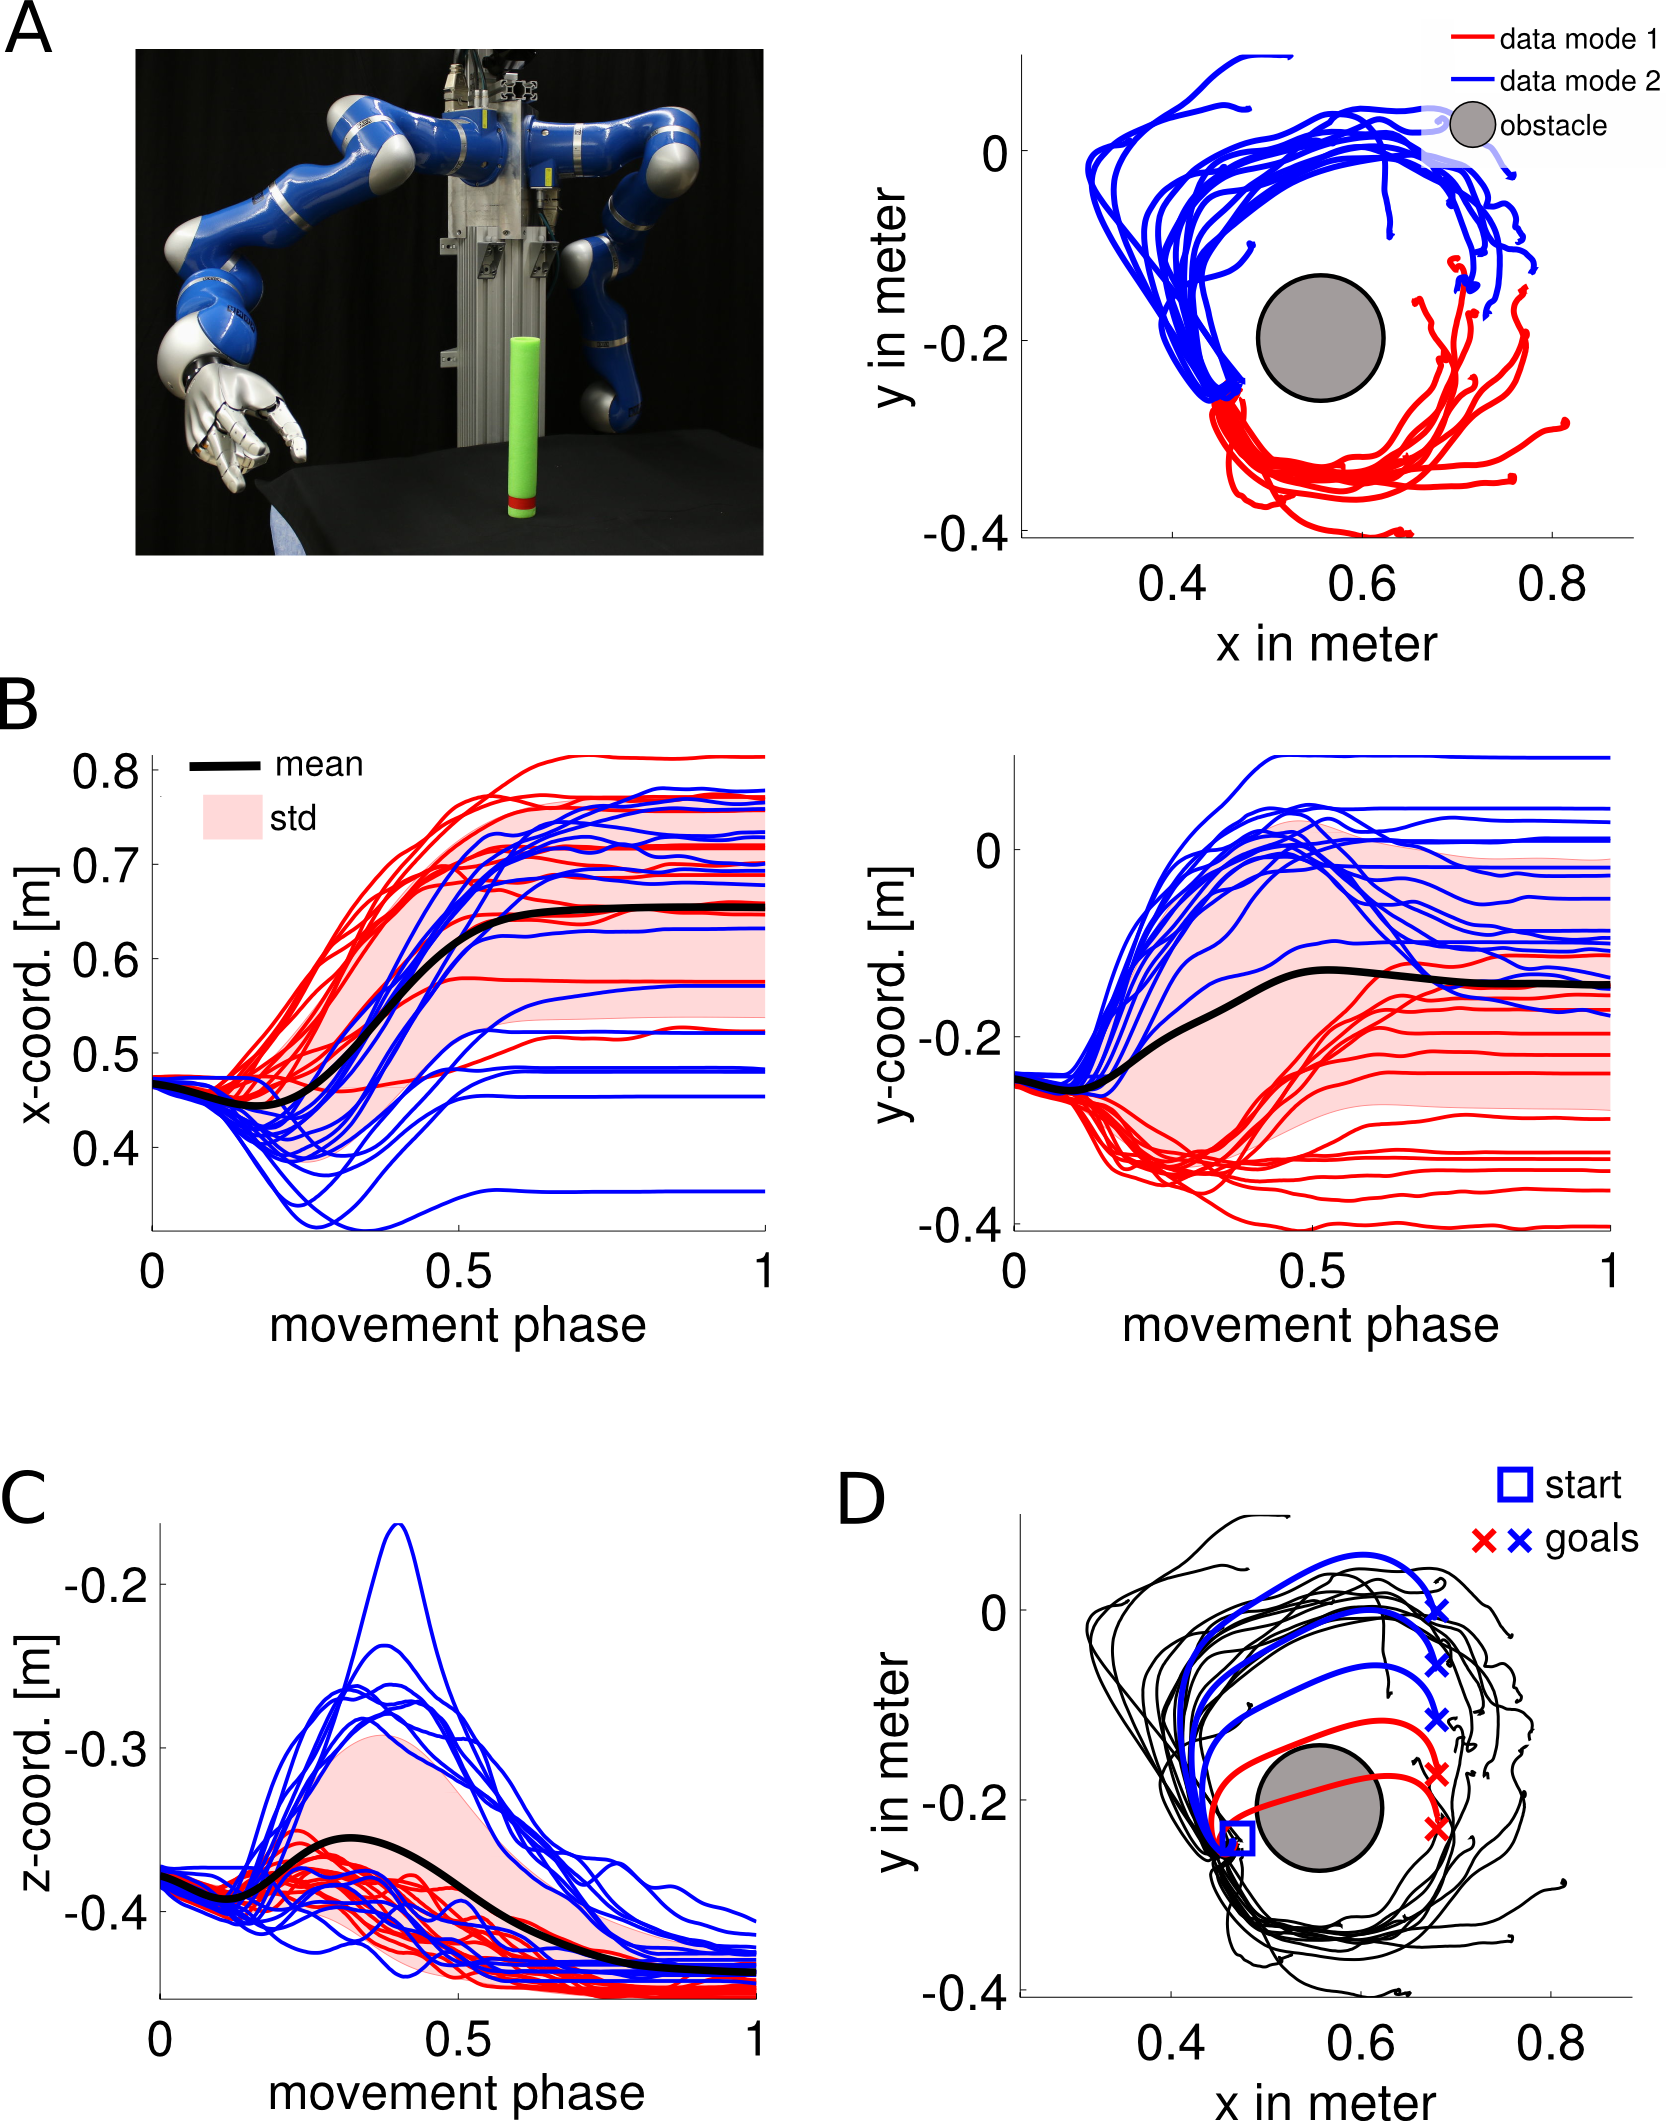
\includegraphics[width=0.9\columnwidth]{BiModal_Data_ProMPs.png}
\end{center}
\caption{(A) Experimental setting and two dimensions out of the $7$-dimensional dataset (three end-effector coordinates and the four dimensional quaternions). The colors (red and blue) denote the movement direction to avoid the obstacle.
(B-C) Learned distributions using ProMPs. The mean is denoted by the black line and the standard deviation by the shaded region. 
ProMPs cannot represent the bi-modal distribution in the $2$nd panel in (B) and 
the conditioning on unseen targets might fail (D). 
\label{fig:bimodal_data_promps}}
%\vspace{-0.5em}
\end{figure}
  
In contrast, the LMProMPs model is able to capture the two modes of the
demonstrations, as shown in Fig. \ref{fig:bimodal_mixture}. We initialized the
experiment with \textit{K-means} clustering method using two components.  The
learned prior distribution and the influence of the first two dimensions of the
latent variable are illustrated in Fig. \ref{fig:bimodal_mixture}(A-B).
Each mixture component specializes on one mode of the data.  Using the learned
bi-modal prior distribution, our model is able to generate trajectories to new 
target locations that avoid the obstacle as shown in Fig.
\ref{fig:bimodal_mixture}(C).  
The inferred trajectories are smooth and can be
executed on the real robot using inverse kinematics to obtain a reference joint
trajectory and inverse dynamics control to execute it.  The resulting
trajectories of the end-effector of the real robot are illustrated in Fig.
\ref{fig:bimodal_mixture}(D). 


%The results for the hierarchical prior model are shown in Fig. \ref{fig:bimodal_mixture}, 
%where in this first experiment the model was initialized with the \textit{kmeans} method using two components. 
%The learned prior distribution and the influence of the first two dimensions of the latent 
%variable are illustrated in Fig. \ref{fig:bimodal_mixture}(A-B). 
%Each mixture component specializes on one mode of the data. 
%Using the learned bi-modal prior distribution, 
%the model is able to generate new trajectories to unseen target locations that avoid the obstacle as shown in Fig. \ref{fig:bimodal_mixture}(C). 
%The inferred trajectories are smooth an can be executed on the real robot using inverse kinematics control. 
%The resulting trajectories of the end-effector are illustrated in Fig. \ref{fig:bimodal_mixture}(D). 

\begin{figure}%[!t]
\begin{center}
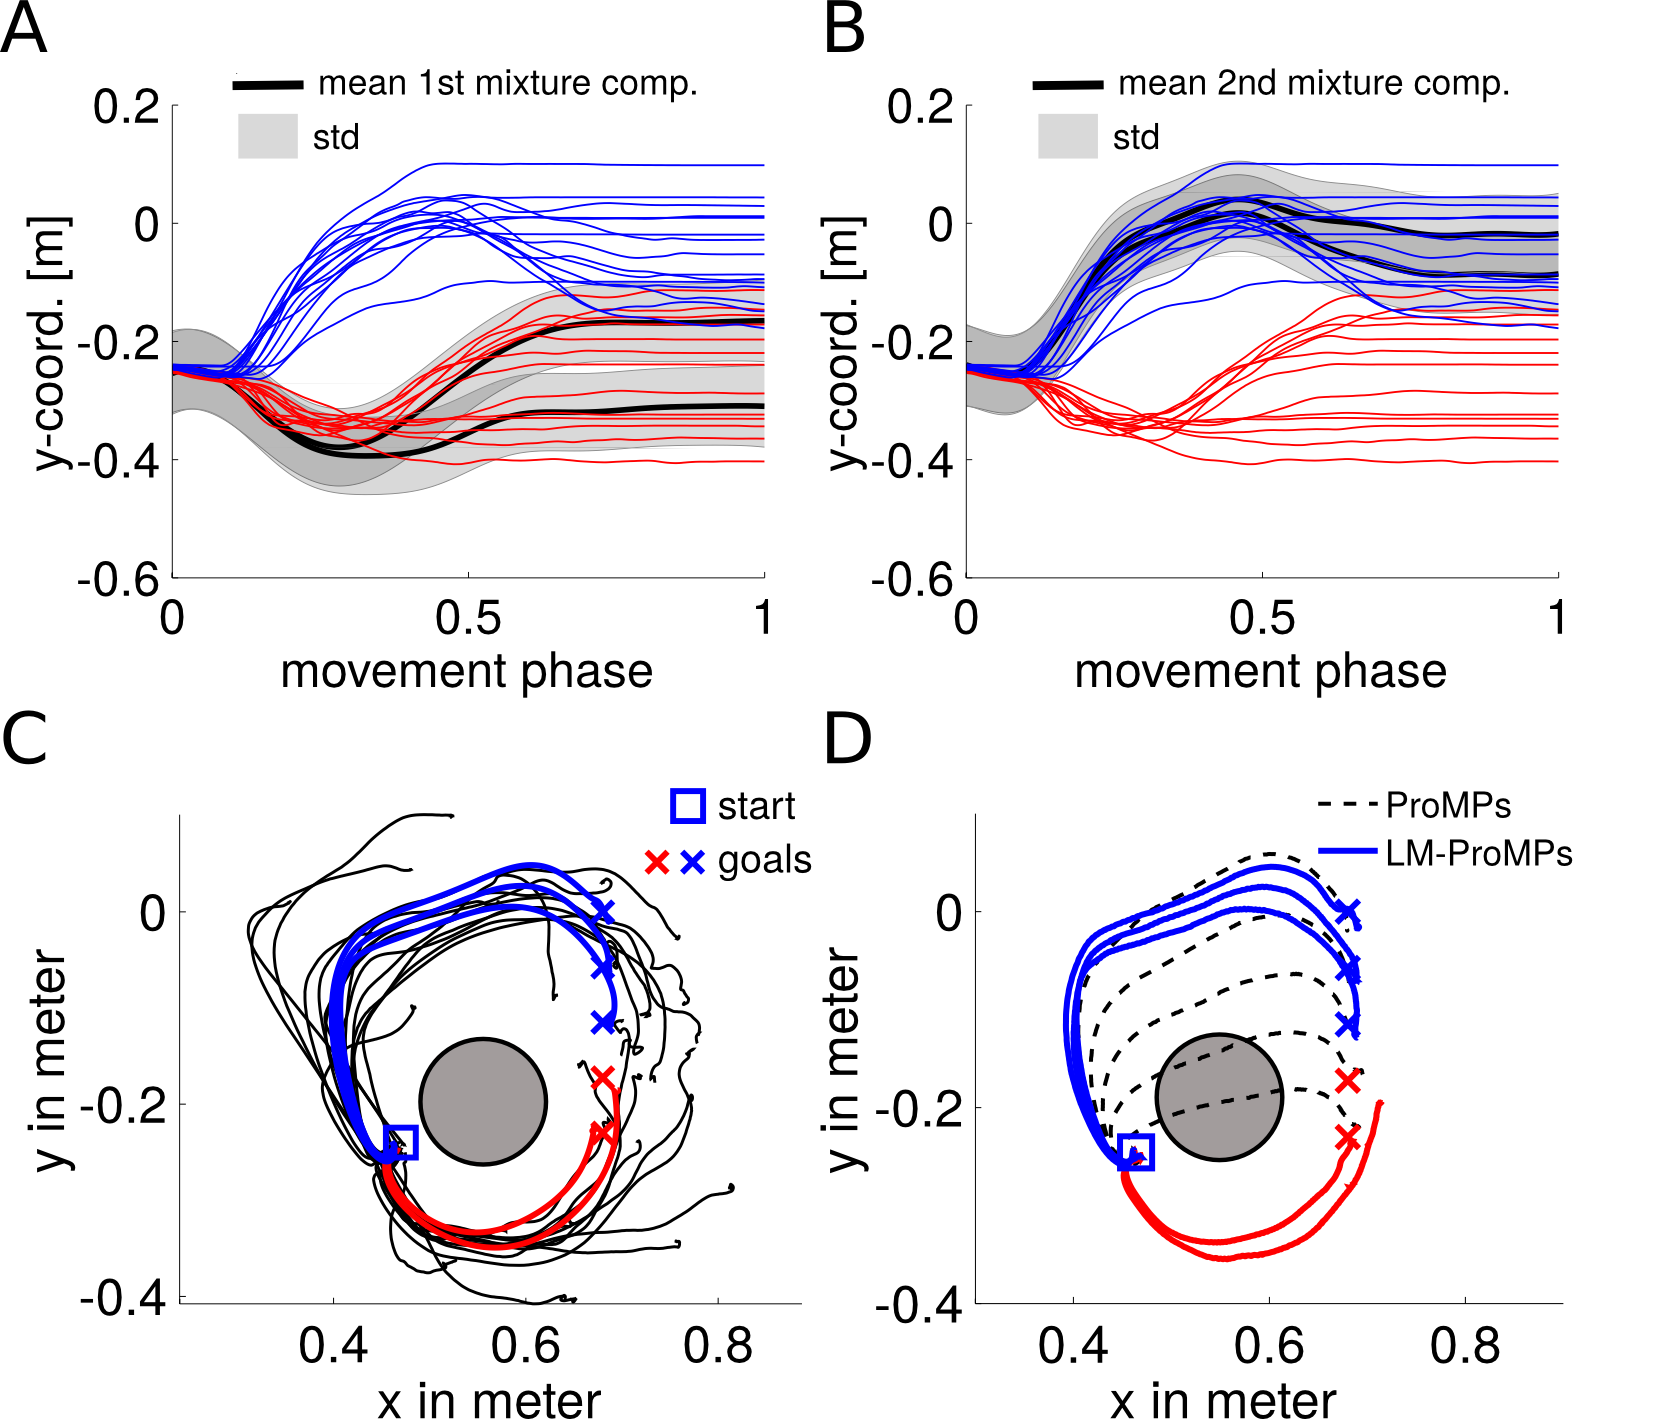
\includegraphics[width=0.9\columnwidth]{BiModal_Mixture.png}
\end{center}
\caption{Learned bi-modal distribution (the colors red and blue denote the modes) using the proposed mixture model with two mixture components (A-B). 
The latent variable is used to specialize on subregions within the distribution of the mixture component. 
This is illustrated for two dimensions of $\textbf{h}$, where solid black lines denote the mean. 
(C) Conditioning result using LMProMPs. (D) Real robot results.
\label{fig:bimodal_mixture}}
%\vspace{-0.5em}
\end{figure}
  
